\subsubsection{Spannungsverstärkung}
Die Werte zur Bestimmung der Spannungsverstärkungen wurden bei einer
Eingangsspannung von $U_{\mathrm{RMS}} = 5 \, \si{\milli\volt}$ und einer
Frequenz von $f_e = 1 \, \si{\kilo\hertz}$ bestimmt. Der Lastwiderstand wurde
von $100 \, \si{\kilo\ohm}$ bis $1 \, \si{\kilo\ohm}$ variiert. Die
Spannungsverstärkungen bei den jeweiligen Lastwiderstandswerten ist dann
derQuotient aus Ausgangs- und Eingangsspannung. Die Spannungswerte wurden
als RMS-Werte am Oszilloskop gemessen. Der interne Lastwiderstand beträgt $R_{\mathrm{L,intern}} =
100 \, \si{\kilo\ohm}$.

\begin{table}[H]
  \begin{center}
    \begin{tabular}{|c|c|c|c|}
      $U_e / \si{\milli\volt}$ & $U_a / \si{\milli\volt}$ & $R_{\mathrm{L,gesamt}} / \si{\kilo\ohm}$ & $V_u$\\
      \hline
      \hline

      4.99 & 810.96 & 100 & 162.5\\
      4.97 & 790.5 & 33.33 & 159.1\\
      4.98 & 721.6 & 9.09 & 144.90\\
      4.97 & 363,9 & 0.99 & 73.22\\
      \hline
    \end{tabular}

  \end{center}

  \caption{RMS-Spannungswerte und daraus resultierende Verstärkung bei
    verscheidenen Lastwiderständen}

\end{table}

\begin{figure}[H]
  \begin{center}
    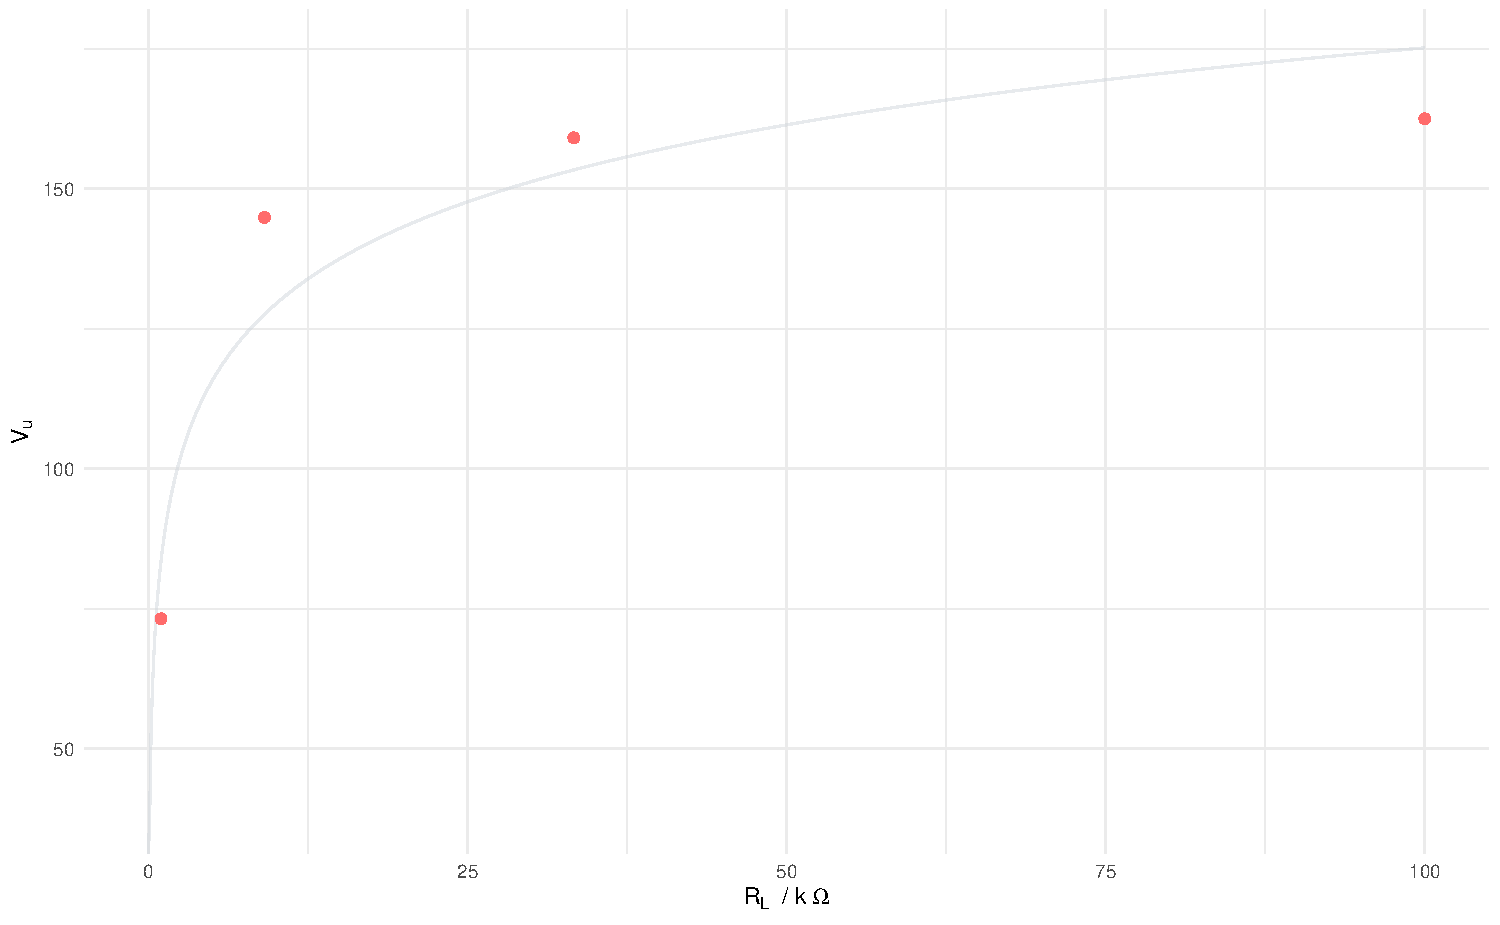
\includegraphics[width=\textwidth]{2_3/2_3_1.pdf}
  \end{center}
  \caption{Graph der Messwerte}
\end{figure}

Der Anstieg des Graphen entspricht der Steilheit $g_m$ des Transistors. Die
Steilheit im Arbeitspunkt ist etwa
\[g_m = \frac{I_C}{U_T} = \frac{4.33 \, \si{\milli\ampere}}{26 \,
    \si{\milli\volt}} = 188.26 \, \si{\milli\siemens}\]

Der theoretische Zusammenhang ist
\[V_u = - g_m \cdot R_L \] 

Der scheinbar lineare Zusammenhang ist aus dem Messwertgraphen jedoch nicht
erkennbar. Dies liegt daran, dass der interne Kollektorwiderstand $R_3$ als
Parallelschaltung in den Gesamtlastwiderstand eingeht.
\[V_u = -g_m \cdot R_3 // R_{\mathrm{L,extern}}\]

$R_3 = 1.3 \, \si{\kilo\ohm}$ legt hier durch die Parallelschaltung den
theoretischen Grenzwert der Spannungsverstärkung fest. \[|V_{u,max}| = 188.26 \,
  \si{\milli\siemens} \cdot 1.3 \, \si{\kilo\ohm} \approx 245\]


Bei hohen externen Widerstandswerten dominiert der Widerstand $R_3$ in der
Parallelschaltung, wodurch der Gesamtlastwiderstand etwa $R_3$ ist, die
Verstärkung läuft gegen einen konstanten Wert.
Bei geringen Widerstandswerten muss die Parallelschaltung berücksichtigt
werden.

Durch Berücksichtung des Kollektorwiderstandes erhält man dann den erwarteten Zusammenhang.

\begin{figure}[H]
  \begin{center}
    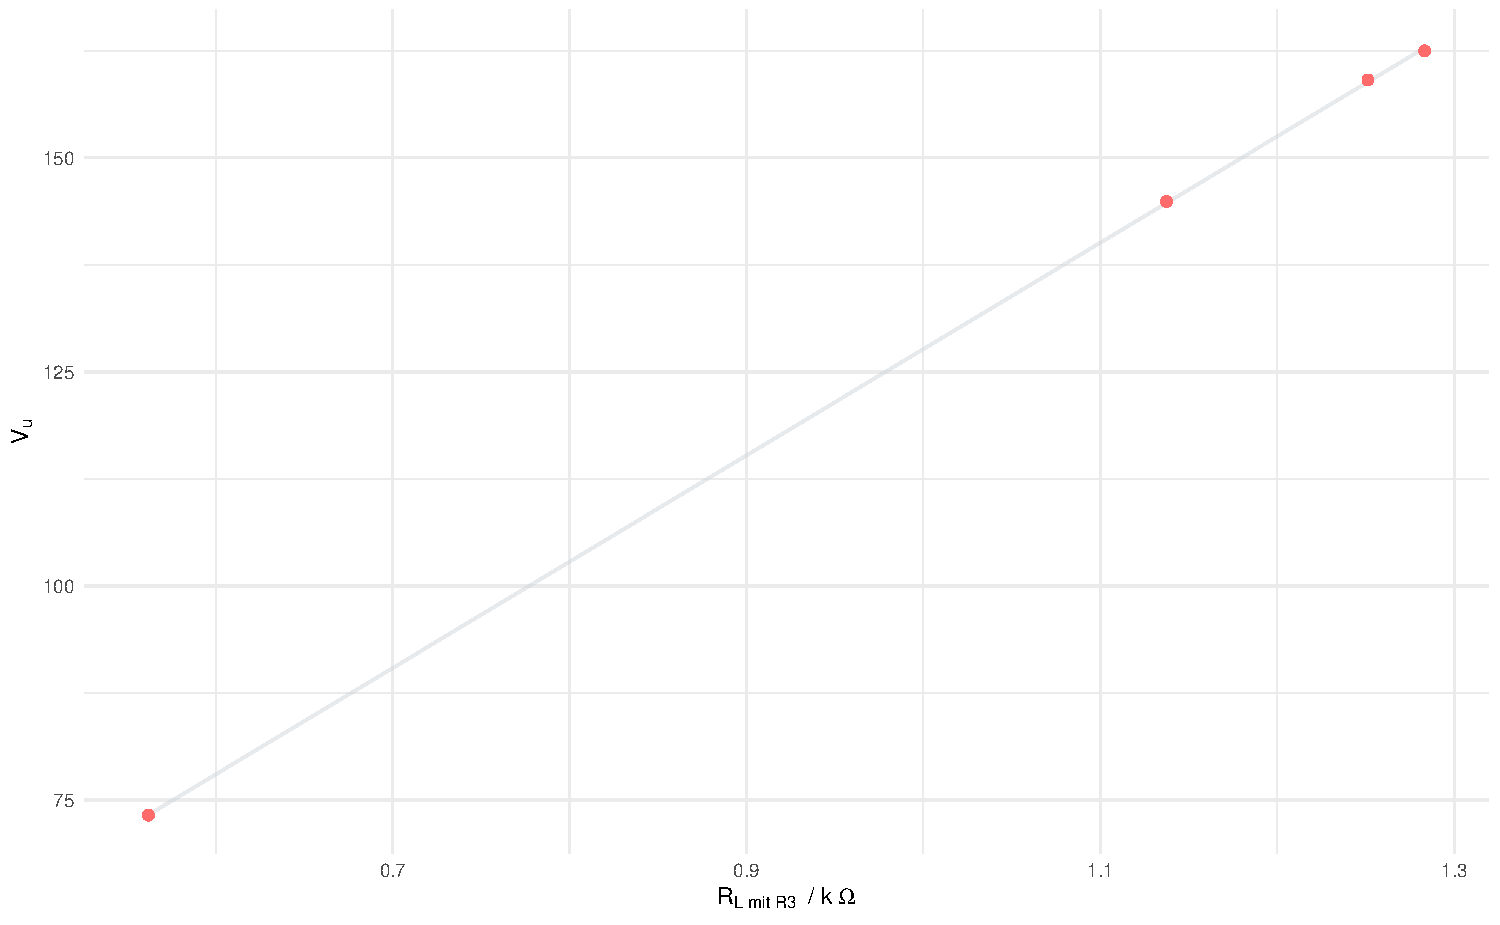
\includegraphics[width=\textwidth]{2_3/2_3_1_corrected.pdf}
  \end{center}
  \caption{Graph der Messwerte, korrigiert}
\end{figure}

Die resultierende Steilheit ist somit:
\[g_m \approx 128 \, \si{\milli\siemens}\]


(Da die Eingangsspannung den Kollektorstrom jedoch etwas verschiebt, ist die
Steilheit nicht konstant, was zu einer Abweichung des theoretisch linearen
Verhaltens führt. Außerdem wurde der Ausgangswiderstand des Transistors nicht berücksichtigt)

\subsubsection{Eingangswiderstand}
Mithilfe der U/2-Methode wurde der Eingangswiderstand der Schaltung bei
konstantem Lastwiderstand von $100 \, \si{\kilo\ohm}$ (kein externer Widerstand)
und einer Frequenz von $1 \, \si{\kilo\hertz}$ bestimmt.

\[U_{a1} = \frac{U_a}{2} = 413 \, \si{\milli\volt}\]

Der dabei ermittelte Eingangswiderstand ist
\[r_e = 800 \, \si{\ohm}\]

\subsubsection{Ausgangswiderstand}
Der Ausgangswiderstand bestimmt sich über die umgestellte Spannungsteilerformel
am Ausgangskreis. $U_{a0}$ ist die Leerlaufspannung, ohne Belastung. $U_{a1}$
die Ausgangsspannung bei Belastung mit $R_L$.
\[U_{a1} = U_{a0} \cdot \frac{R_L}{r_a + R_L}\]
\[r_a = R_L \left( \frac{U_{a0}}{U_{a1}} -1 \right)\]

\[U_{a0} = 821.45 \, \si{\milli\volt}\]
\[U_{a1} = 731.50 \, \si{\milli\volt}\]

\[r_a = 100 \, \si{\kilo\ohm} \left( \frac{ \, \si{\milli\volt}}{\,
      \si{\milli\volt}} -1 \right) = \, \si{\kilo\ohm}\]


\subsubsection{Amplituden-Frequenzgang}
Der Amplituden-Frequenzgang wurde durch das Durchlaufen der
Eingangsspannungsfrequenzen von $0$ bis $10 \, \si{\kilo\hertz}$ und die Messung
der Ausgangsspannungswerte (RMS) bei einer Eingangsspannung von $U_e =
5\,\si{\milli\volt}_{\mathrm{RMS}}$ ermittelt.

\begin{figure}[H]
  \begin{center}
    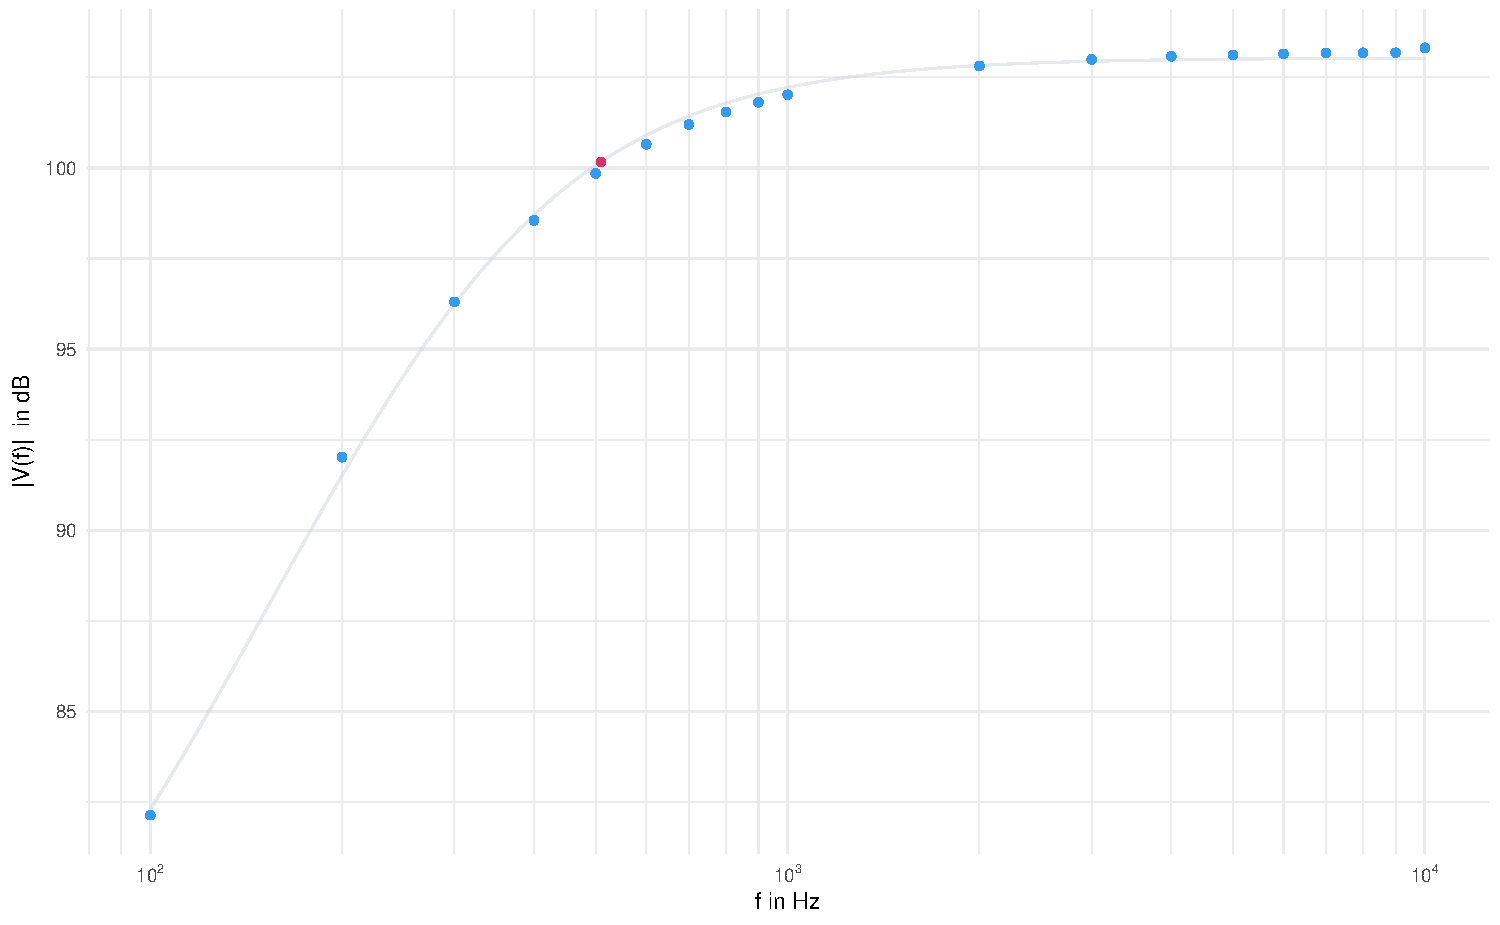
\includegraphics[width=\textwidth]{2_3/2_3_frequenzgang.pdf}
  \end{center}
  \caption{Amplitudenfrequenzgang der Messung}
\end{figure}

Die durch Regression ermittelte Grenzfrequenz ist
\[f_g = 500 \, \si{\hertz}\]

Vor der Grenzfrequenz steigt die Verstärkung mit etwa $25 \, \si{\deci\bel}$ pro
Dekade. Weit hinter der Grenzfrequenz nimmt sie den entsprechenden Wert aus
2.3.1 an.

$C_E$ ($C_3$) stellt wechselstromseitig einen Kurzschluss dar, wodurch der
Emitterwiderstand diesbezüglich wegfällt und die Verstärkung für 
Wechselspannungen deren Frequenz hoch genug ist nicht beeinflusst. Bei
niedrigeren Frequenzen ist die Reaktanz des Kondensators jedoch nicht
ausreichend gering, um den Einfluss von $R_E$ vollständig zu beseitigen.